\chapter{Covariates Affecting Densities and Detectability}\label{Chap7}

\section{Reasons to Include Covariates} \label{sec:Chap7}

In previous chapters, we illustrated how an individual-based process where each individual has marks representing demographic variables (i.e., a marked point process from a Lagrangian viewpoint) can be approximated as gridded densities (i.e., an Eulerian viewpoint) and fitted as a generalized linear model (GLM).  We have also shown how residual spatial variation can be modeled by estimating the response to spatial basis functions while integrating across the value of random effects in a generalized linear mixed model (GLMM).  This then allowed us to develop basic types of species distribution models (SDMs), where species encounters, counts, or biomass densities are treated as response variables in a GLMM.  However, we haven't previously emphasized the role of covariates in a GLMM and SDM.

Covariates might be included in an SDM for a variety of different reasons including: 
\begin{itemize}
    \item \textit{Mitigating bias}: the SDM could be fitted to data that differ substantially in measurement methods or sampling protocols.  For example, an ecologist might fit samples of population density using historical (visual) and contemporary sampling methods (environmental DNA), where the mean of each sample is affected both by population density and the characteristics of each sampling method.  In this case, including information about the sampling methods can be used to filter out a portion of variance that is explained by sampling method, and thereby eliminate what would otherwise cause a bias in resulting estimates of population density;
 
    \item \textit{Interpolation}: similarly, the SDM can be fitted and then used to predict species densities at new locations.  If the location of samples is representative of the area being sampled (e.g., they arise from a probability sampling design), then the estimated model is likely representative of other locations in the same spatial domain.  We call this predictive task \myindex{interpolation};
    
    \item \textit{Attribution}\index{attribution}: the SDM can be fitted with a variety of covariates representing environmental or experimental conditions.  If these covariates are truly exogenous (as known strongly in the case of randomized treatments, or sometimes believed in the case of observed covariates), then an estimated response curve can be treated as measuring a causal mechanism.  This then allows researchers to conduct experiments \textit{in silico} to see how a response would have been different under different environmental or experimental conditions, and thereby attribute real-world outcomes to observed conditions;

   \item \textit{Counterfactual evaluation}:  finally, the SDM could be used to predict species densities under novel conditions.  As we will see, this differs from interpolation because it may involve predicting the response to ecological conditions that have never been observed, either because these conditions reflect some new ecological context, human pressure, or experimental treatment.  
\end{itemize}
Both attribution and counterfactual evaluation are tasks that require predicting a response under covariate values that were not directly observed.  Both could perhaps be called \myindex{extrapolation}, and it is often observed that extrapolation is more difficult than interpolation \cite{roberts_cross-validation_2017}.  However, we distinguish two different types of extrapolation, where it is easier to extrapolate to conditions that are fundamentally similar to those previously observed (attribution) than extrapolating to conditions that are in some way different from previous observations (counterfactual predictions). SDM performance when extrapolating to new ecological conditions (which we call counterfactual prediction) is sometimes called \myindex{transferability}, and we will see that ecological knowledge is typically required to hope for transferability.

In this chapter, we will explore how covariates can aid in all of these tasks.  To do so, we will first discuss causal inference and structural equation models in detail.  We will use this discussion to illustrate when conventional regression models will result in biased estimates of the effect of covariates (i.e., misleading attribution) and poor performance under new conditions (i.e., poor counterfactual prediction), and also show when these will be unbiased.  We will then emphasize a distinction between detectability and density covariates, and show how detectability covariates can be used to intercalibrate data from multiple sources. 

\section{Predicting the Effect of System Changes} \label{sec:Chap7_predicting_effect}

\begin{figure}[!ht]
    \caption[Causal map and regression estimates for simplified ecosystem]{The true causal map (left panel) representing mechanisms in a hypothesized soil community with three system variables (boxes) where an arrow indicates a linear causal effect and the number next to each arrow shows the magnitude of response.  For example, the arrow from Temperature to log(Density) indicates that a 0.1-degree increase in Temperature would cause a 10\% increase in Density.  We also show the estimated effect (right panel) when erroneously analyzing data from this ecosystem as a standard generalized linear model.}
    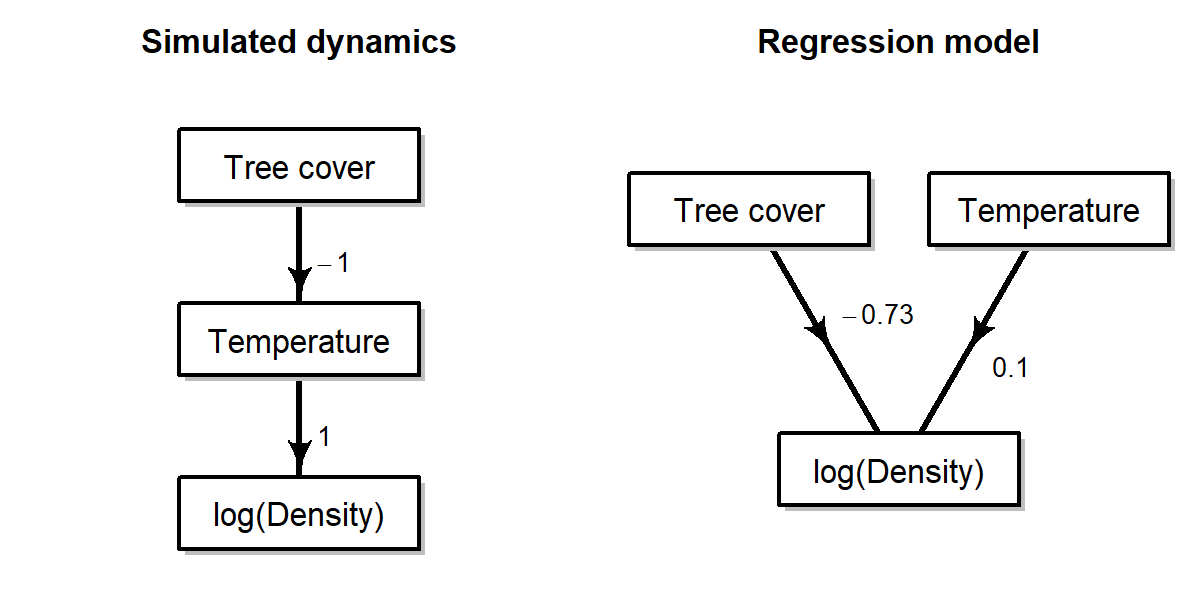
\includegraphics[width=5.5in]{Chap_7/graph.png}
    \label{fig:Chap7_causal_map}
\end{figure}

To begin, imagine a study focused on how the abundance of soil invertebrates \(N\) in a standardized sample is affected by soil temperature \(T\) and tree cover \(C\).  For illustration purposes, we will imagine that soil invertebrate densities increase with increasing soil temperature (due to increased foraging and growth rates), and that soil temperature decreases in areas with high tree cover (due to decreased solar heating and increased evapotraspiration)\footnote{See https://github.com/james-thorson/Spatio-temporal-models-for-ecologists/Chap\_7 for code associated with this chapter.}.  For illustration, we specify parameter values and assume that soil invertebrate densities follow a log-linked Poisson process:

\begin{equation} \label{eq:Chap7_sem_example}
\begin{gathered}
   C \sim \mathrm{Normal}(0,1) \\ 
   T \sim \mathrm{Normal}(-C, 0.1^2) \\
   N \sim \mathrm{Poisson}(e^T)
\end{gathered}
\end{equation}
such that a change in temperature results in a proportional change in log-density.  We visualize these effects using a \myindex{causal map} that represents the causal mechanisms operating in our hypothesized ecosystem (Fig. \ref{fig:Chap7_causal_map} left panel).  This causal map includes:
\begin{itemize}
    \item One box for each variable, without differentiating between those that might be considered response or predictor variables;

    \item One arrow for each direct effect of one variable on another.
\end{itemize}
We specifically construct a causal map with linear effects for each mechanism, and show the \myindex{path coefficient} that represents the strength of each linear effect.  The total effect of one variable \(A\) on another variable \(B\) can then be computed by taking the sum across paths flowing from \(A\) to \(B\), where the effect from each path is computed as the product of path coefficients for each arrow along that path \cite{wright_method_1934}.  In this simplified model, for example, we have only a single path linking tree cover \(C\) to log-densities \(\log(D)\), i.e., \( C \rightarrow T \rightarrow \log(D) \), which implies that C has a linear effect on \(\log(D)\) with a net magnitude of \(1 \times -1 = -1\).

To analyze data resulting from this hypothetical ecosystem, many ecologists have been trained to use a regression model that treats an ecological variable of interest (e.g., soil invertebrate densities) as a response and available ecosystem characteristics (e.g., tree cover, temperature, etc) as covariates.  A sophisticated analyst might then acknowledge that invertebrate counts are non-negative counts and specify a log-linked Poisson distribution, or might additionally use random effects to address pseudoreplication resulting from a nested sampling design.  We therefore fit 100 measurements from this causal map with a generalized linear model of the form \colorbox{backcolour}{glm(N $\sim$  C + T, family=``poisson")}.  

\begin{figure}[!ht]
    \caption[Simulated performance of a GLM when fitting a causal map]{Estimates of the effect of tree cover (top left) and temperature (bottom left) using a GLM \colorbox{backcolour}{glm(N $\sim$ C + T, family=``poisson")}, along with the true values (blue line) from the data-generating process (Eq. \ref{eq:Chap7_sem_example}), and the performance (proportion variance in true log-density explained by predicted log-density) when predicting new data arising from the same data-generating process (top-right panel) or predicting densities under a counterfactual where the temperature has increased by 1 degree Celcius without any change in tree cover (bottom-right panel).}
    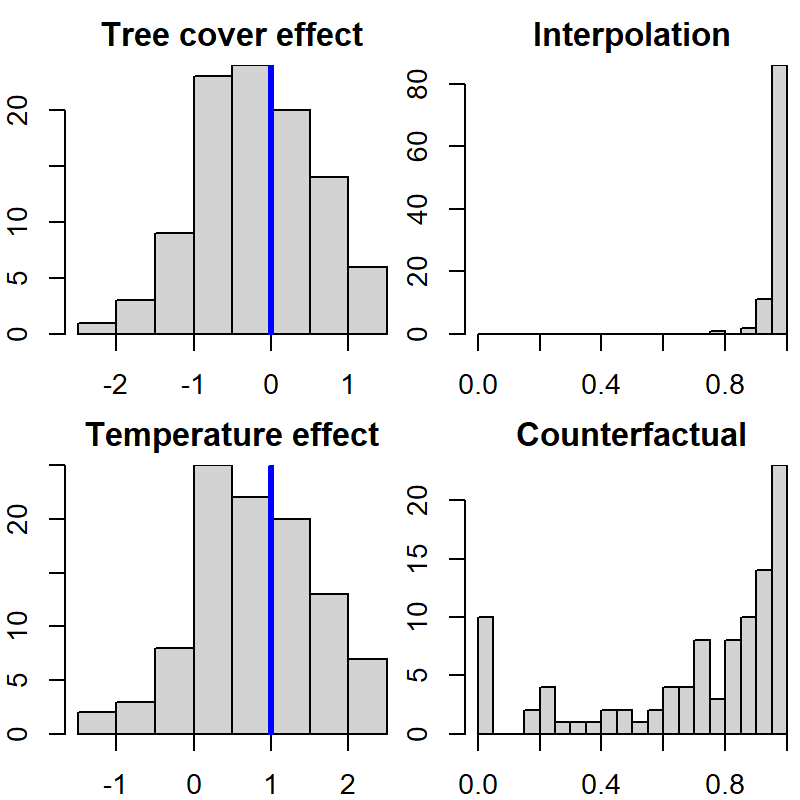
\includegraphics[width=5.5in]{Chap_7/GLM_performance.png}
    \label{fig:Chap7_GLM_performance}
\end{figure}

Fitting this GLM results in poor estimates for both covariates (Fig. \ref{fig:Chap7_causal_map} right panel), where e.g. the estimated effect of Temperature is highly imprecise.  The measured response \(N\) could be correctly modeled using a GLM of the form \colorbox{backcolour}{glm(N $\sim$  T, family=``poisson")} that is nested within the fitted GLM.  Therefore, we are not suprised to see that the estimated Temperature effect is approximately unbiased when we replicate the experiment 100 times (Fig. \ref{fig:Chap7_GLM_performance} left panels).  

Despite being unbiased, estimates of the Temperature effect are highly variable among replicates (e.g., the Temperature effect ranges from \(-1\) to \(3.5\)), and standard errors are extremely large in any single experiment.  Standard errors are large because the two modeled covariates (Tree Cover and Temperature) are highly (\(-0.99\)) correlated, and this is called \myindex{collinearity} when both are included in the same regression model.  It might surprise some readers, however, to see that collinearity does not degrade extrapolation-performance when predicting soil invertebrate densities for 100 new locations with temperature and tree cover drawn from the same underlying process (Fig. \ref{fig:Chap7_GLM_performance}, top right panel).  However, we also simulate new data from the same model, but where temperatures have increased by 1 degree Celcius relative to their average in the fitted data without any change in tree cover (e.g., due to climate change that was not represented in the historical data  available to estimate parameters).  In this counterfactual scenario, the fitted GLM then has substantially degraded performance for predicting soil invertebrate densities under novel conditions (Fig. \ref{fig:Chap7_GLM_performance}, bottom right panel). One interpretation for this degraded performance is that the structure of collinearity has changed between the fitted and predicted samples \cite{dormann_collinearity_2013}.

From this simple example we can draw several lessons that are also true of causal inference in general:

\begin{enumerate}
     \item Inference about the effect of covariates is hugely benefited by (or depends upon) a correct understanding of any causal mechanisms that link those covariates;
     
     \item Fitting to multiple covariates that are correlated (\textit{collinearity}) will typically result in imprecise estimates of slopes in a regression model, but predictions can still be accurate when using collinear variables as long as the relationship among covariates during predictions are similar to those occurring in the fitted data;

     \item Predicting the consequences of counterfactual changes in covariates is highly sensitive to the specified relationship among covariates (the \textit{causal map}).
\end{enumerate}

Given these conclusions, we next introduce \myindex{do-calculus} as an general and comprehensive vocabulary for thinking about the effect of covariates in ecological models, and use this to discuss structural equation models (SEM) as a potential solution to these issues.  

\subsection{Do-calculus and Causal Inference} \label{sec:Chap7_do-calculus}

All scientists are trained to understand that \textit{correlation does not imply causation}, i.e., that identifying two correlated variables does not imply that a change in one will cause a change in the other.  Similarly, scientists are typically trained to understand that randomly assigning sampling units to alternative experimental treatments and measuring the outcome (a \myindex{randomized controlled experiment} and its variants) is the gold-standard for inferring mechanisms (which we will call \myindex{causal inference}).  However, there is less general understanding and agreement about when observational data can be used to infer causality, or how to identify those variables that must be measured when a system cannot be manipulated experimentally due to logistical or ethical constraints.  

To address these and other questions about causal inference, we briefly review the literature regarding \myindex{do-calculus} \cite{pearl_causal_2009,pearl_causality_2009}.  In essence, this literature defines a \textit{do-operator}, where this do-operator then defines the value or distribution of variables \(B\) as if other variables \(A\) have been exogenously fixed at some hypothetical value or distribution.  In particular, we can write the distribution for \(B\) as \(B| \mathrm{do}(A=a_{new})\) when covariates are fixed at value \(a_{new}\) or \(B| \mathrm{do}(A=A_{new})\) when covariates are fixed at distribution  \(A_{new}\).  We can fit a probabilistic model, and then use these estimated distributions for three types of analysis \cite{pearl_causal_2009}:
\begin{enumerate}
    \item \textit{Policy evaluations}: We can calculate the distribution for a given response \(B | \mathrm{do}(A=A_{policy}) \) under alternative assumptions about an exogenous policy choice \(A_{policy}\).  This allows us to identify an efficient policy by optimizing the outcome with respect to that policy;

    \item \textit{Attribution}: We can calculate the probability of an observed event under scenarios that differ from those that really occurred, and use this to calculate how real-world conditions either increased or decreased this probability relative to some baseline probability.  This then allows us to identify what past conditions were responsible for an increased or decreased probability of a past event. This type of probabilistic attribution has seen increased use in policy discussions of climate change and its effect on extreme weather events \cite{naveau_statistical_2020};  

    \item \textit{Mediation analysis}:  Returning to our soil community example, let us imagine that \( C \rightarrow T \rightarrow \log(D)\) and also \(C \rightarrow \log(D)\). In this expanded example, we see that tree cover \(C\) has a direct effect on log-density \(\log(D)\) and also has an indirect effect that is mediated by Temperature \(T\).  We might then want to know what fraction of the effect of \(C\) on \(\log(D)\) is due to mediator variable \(T\).  This \textit{mediation analysis} then provides insight into the proximal mechanisms that underlie large-scale correlations. 
\end{enumerate}

In our previous example, we defined a joint distribution for three variables \( \Pr(C,T,\log(D)) \) where sampled abundance was a noisy measure of log-density \(\log(D)\).  In the causal map defined for the simulation experiment, we then decompose this joint distribution:

\begin{equation}
    \Pr(C,T,\log(D)) = \Pr(\log(D)|T) \times \Pr(T|C) \times \Pr(C)
\end{equation}
i.e., where log-density \(\log(D)\) is independent of tree cover \(C\) conditional upon the value of temperature \(T\) (and see Section \ref{sec:Chap2_Hessian_sparsity} for more discussion of conditional independence and graphical models).  However, this probability notation is ambiguous about how to interpret an experiment where temperature \(T\) is changed to a new value.  This change in temperature could perhaps represent:
\begin{itemize}
    \item An \textit{endogenous} change, wherein tree cover \(C\) is changed exogenously (i.e., due to changing land management or fire regimes), and this causes an endogenous change in temperature \(T\) and then a resulting change in soil densities \(\log(D)\);

    \item An \textit{exogenous} change, wherein some un-modeled variable (i.e., an experimental treatment, or global climate change) causes a change in temperature \(T\) even though tree cover \(C\) is unchanged, via a causal pathway that is not explicitly represented in the causal map.
\end{itemize}
Importantly, the endogenous change in \(T\) is then represented using do-calculus as:

\begin{equation}
    \Pr(C,T,\log(D)) = \Pr(\log(D)|T) \times \Pr(T|\mathrm{do}(C=C_{new}))  
\end{equation}
where the distribution \(\Pr(T|\mathrm{do}(C=c_{new}))\) results from an exogenous change in \(C\) to value \(c_{new}\).  Alternatively, the exogenous change in \(Y\) is represented using do-calculus as:

\begin{equation}
    \Pr(C,T,\log(D)) = \Pr(\log(D)|\mathrm{do}(T=T_{new})) \times \Pr(C) 
\end{equation}
where \(T_{new}\) represents some new distribution that arises from mechanisms that are not represented in the probability distribution (i.e., an experiment, or some other exogenous change), and hence does not affect the distribution for \(C\).

As we have seen in Fig \ref{fig:Chap7_GLM_performance}, fitting a regression model to covariates that have a complicated mechanistic relationship can result in biased or imprecise predictions when covariates are then changed exogenously.  Unfortunately, this scenario is precisely what ecologists are often asked to do, i.e., to predict changes resulting from exogenous changes in global climate, human behavior, and introduced species.  We therefore present one approach to addressing this issue, i.e., using a structural equation model that explicitly represents mechanisms among covariates.

\subsection{Structural Equation Models} \label{sec:Chap7_strutural_equation_models}

We next demonstrate these concepts in detail by introducing structural equation models\index{structural equation model} (SEM).  We demonstrate how SEM can be used to model the correlation among covariates as well as their effect on a response variable, and also how this can be used during extrapolation to conduct both attribution and counter-factual prediction.  Recall that in Section \ref{sec:Chap4_SEM}, we defined a structural equation model as providing a distribution for a vector of variables \( \mathbf{y} \), e.g., \( \mathbf{y} = (C, T, \log(D)) \).  Unlike a standard regression, none of these variables are defined as predictor or response variables;  instead, we define endogenous and mechanistic relationships among variables using a matrix of path coefficients \( \mathbf{\Rho} \), and also define exogenous variation \( \mathbf{\delta} \) which follows covariance \( \mathbf{\Sigma = \Lambda \Lambda}^t \).  

\begin{equation} \label{eq:Chap7_SEM_process}
\begin{gathered}
    \mathbf{y} = \mathbf{\Rho y} + \mathbf{\delta}  \\
    \mathbf{\delta} \sim \mathrm{MVN}(\mathbf{0},\mathbf{\Sigma})
\end{gathered}
\end{equation}
This then defines the covariance among variables \(\mathbf{y}\):

\begin{equation} \label{eq:Chap7_SEM_covariance}
    \mathrm{Var}(\mathbf{y}) = \mathbf{V} =  \mathbf{B} \mathbf{\Sigma} \mathbf{B}^T    
\end{equation}
where \( \mathbf{B} = (\mathbf{I-\Rho})^{-1} \).  We now can see that this SEM equation and the resulting covariance (Eq. \ref{eq:Chap7_SEM_process} and \ref{eq:Chap7_SEM_covariance}) has similar structure to the simultaneous autoregressive (SAR) process that can be used to calculate the covariance resulting from a spatial or temporal model (e.g., Eq. \ref{eq:Appendix_SAR_process} and \ref{eq:Appendix_SAR_covariance} in Section \ref{sec:Appendix_SAR}).  

Alternatively, we could fit a model that explains the covariance among variables \(\mathbf{v}\) but instead estimates the covariance directly \(\mathrm{Var}(\mathbf{y}) = \mathbf{V}\) as an unstructured matrix, i.e., by estimating parameters in the lower-triangular Cholesky matrix \(\mathrm{L}\) where \(\mathbf{V = LL}^t\) (see Section \ref{eq:Chap4_covariance_matrices}). After estimating parameters for this unstructured covariance matrix, we could then make predictions about values that are missing at random, and summarize relationships between variables by calculating the eigendecomposition of \(\mathbf{V}\) and visualizing the slope of the first couple eigenvectors (called \myindex{major axis regression}) \cite{thorson_predicting_2017, warton_bivariate_2006}.  However, SEM offers several advantages relative to estimating this unstructured covariance among parameters.  We introduced some of these advantages previously in Section \ref{sec:Chap4_SEM}, and here emphasize in particular the justifications labeled \textit{Parsimonious representation} and \textit{Path coefficients as regression slopes}.  However, we now have sufficient context to add a fifth justification, i.e., that SEM provides a natural approach to implementing calculations involving the do-operator (Sec. \ref{sec:Chap7_do-calculus}).  Specifically, if we want to implement a policy evaluation, attribution exercise, or mediation analysis that involves changing a variable \(A\) to a new value or distribution \(A_{new}\), we specify that distribution \( \mathrm{do}(A=A_{new}) \) and then trace impacts along arrows pointing from that variable to other modeled variables \cite{pearl_causal_2009,wright_method_1934}.  We therefore add this to the list from Sec \ref{sec:Chap4_SEM}:
\begin{enumerate}
    \item[5] \textit{Clarify how to do counter-factual analyses}:  fitting an SEM provides a natural way to conceptualize and compute the expected impact of changing one variable on downstream variables.   
\end{enumerate}
In particular, we might seek to predict the consequences of an exogenous change in the vector of state variables from \(\mathbf{y}_0\) to \(\mathbf{y}_0 + \Delta\).  Exogenous change \(\Delta\) might be an indicator vector (i.e., a vector of zeros except one nonzero element corresponding to the single variable that is changed) or it might represent some simultaneous change in all variables (i.e., all elements of \(\Delta\) are nonzero).  This change \(\Delta\) then causes a first-order change of \(\Rho \Delta\) in other variables (see the first line in Eq. \ref{eq:Chap7_SEM_process}), then a second-order change of \(\Rho^2 \Delta\), and so on.  The total effect of change \(\Delta\) is then calculated by summing across these first, second, and higher-order effects.  Assuming that this power-series is stationary (i.e., the effect of an exogenous change does not grow exponentially as it moves through the estimated system of equations), we can calculate the total effect as:

\begin{equation} \label{eq:Chap7_total_effect}
    \sum_{n=0}^{\infty} \Rho^n \Delta = (\mathbf{I-\Rho})^{-1} \Delta
\end{equation}
To understand this, let us first assume that the system of equations is not \textit{recursive}, i.e., there are no loops like \(A \rightarrow B \rightarrow C \rightarrow A\) (such that \(\Rho\) can be re-ordered as a lower-triangle matrix).  In this case, Eq. \ref{eq:Chap7_total_effect} reduces to calculating the total effect of \(A\) on \(C\) by summing across paths flowing from \(A\) to \(C\), where each path is the product of path coefficients for arrows along that path. In the notation of do-calculus for non-recursive systems, we can therefore use Eq. \ref{eq:Chap7_total_effect} to compute \(\Pr(C | \mathrm{do}(A=A+\Delta_A, B=B+\Delta_B))\) where \(\Delta_A\) and \(\Delta_B\) are the exogenous changes to variables \(A\) and \(B\).  However, Eq. \ref{eq:Chap7_total_effect} can also be computed for recursive systems, where computing the total effect is otherwise less straightforward.  

\lstset{style=Rcode} 
\lstinputlisting[language=R, firstline=112, lastline=120, label=code:Chap7-build-ram, caption=R code to specify parameters in a SEM using the arrow notation that is then parsed by \colorbox{backcolour}{sem::specifyModel} and subsequently passed to TMB., captionpos=t]{Chap_7/Demo_path_diagram.R}

To estimate parameters for the causal map in Fig. \ref{fig:Chap7_causal_map}, we first define the model using the textual interface from R-package \colorbox{backcolour}{sem} \cite{fox_sem_2020}, which is itself based upon common notation for defining path-analysis models \cite{wright_analysis_1934}.  We used this notation previously to illustrate parsimonious specification of the covariance in movement among animals (Section \ref{Section:Chap4_comparing_factor_and_SEM}) but review the notation again here.  This text interface requires the user to specify:
\begin{enumerate}
    \item A one-headed arrow, e.g., \colorbox{backcolour}{A -$>$ B} to specify that a change in variable A from \(A=A_0\) to \(A=A_0 + \Delta\) is expected to cause B to change from \(B=B_0\) to \(B = B_0 + \rho \Delta\), where \(\rho\) is an estimated parameter in path matrix \( \mathbf{\Rho} \);

    \item A two-headed arrow to specify variance (e.g., \colorbox{backcolour}{A $<$-$>$ A}) or covariance (e.g., \colorbox{backcolour}{A $<$-$>$ B}) parameters that are then estimated in matrix \( \mathbf{\Lambda} \);

    \item A name for the parameter associated with each one-headed or two-headed arrow, e.g., \colorbox{backcolour}{b1} or \colorbox{backcolour}{b2}, and any two parameters that have the same name are assumed to also have the same value;

    \item Which parameters are fixed at some value a priori and not subsequently estimated, where the user can name any parameter \colorbox{backcolour}{NA}, in which case they are assigned the value that immediately follows that name.
\end{enumerate}
We then use the custom function \colorbox{backcolour}{build\_ram} to convert this input format to a matrix that lists all structural parameters in the SEM, where this matrix can then be interpreted in TMB to build covariance \(\mathbf{V}\) from estimated parameters.  We specify \colorbox{backcolour}{endog$.$variances = TRUE } as a shortcut to also estimate a variance parameter in \( \mathbf{\Lambda} \) for every variable that was not explicitly assigned one.  For example, to specify the SEM on the left-hand-side of Fig \ref{fig:Chap7_causal_map}, we specify (Code \ref{code:Chap7-build-ram}) a path coefficient from \(C\) to \(T\) named \colorbox{backcolour}{b1} and a second path coefficient from \(T\) to \(\log(D)\) named \colorbox{backcolour}{b2}. In this model, we will specify a log-linked Poisson distribution for measured response \(N\), and this Poisson distribution represents all exogenous variation in the response.  We therefore ``turn off" exogenous variation for \(\log(D)\) estimated in the covariance term \(\mathbf{V}\) by fixing the estimate of additional variation at 0.01 a priori (i.e., using the line \colorbox{backcolour}{logD $<$-$>$ logD, NA, 0.01}).  In this case, this text file results in the following RAM matrix, which prescribes the parameters to be estimated:

%\verbatiminput{Chap_7/RAM.txt}
\lstset{style=Routput}
\lstinputlisting[language=R]{Chap_7/RAM.txt}
where column \colorbox{backcolour}{heads} indicates whether a parameter is in \(\mathbf{\Gamma}\) or \(\mathbf{\Rho}\), \colorbox{backcolour}{to} and \colorbox{backcolour}{from} indicate the row and column numbers of those matrices defined by a given row, \colorbox{backcolour}{parameter} lists the parameter number, and \colorbox{backcolour}{start} provides a user-specified starting value.  The latter is particularly important for any parameters where \colorbox{backcolour}{parameter=0} in the RAM matrix, indicating that this parameter is turned off.  

In this case, we are estimating:
\begin{equation} \label{eq:Chap7_RAM}
    \mathbf{\Rho} = \begin{bmatrix}
    0 & 0 & 0 \\
    \theta_1 & 0 & 0 \\
    0 & \theta_2 & 0 \\
    \end{bmatrix} 
\end{equation}
and:

\begin{equation} 
    \mathbf{\Lambda} = \begin{bmatrix}
    \theta_3 & 0 & 0 \\
    0 & \theta_4 & 0 \\
    0 & 0 & 0.01 \\
    \end{bmatrix} 
\end{equation}
where this specification involves estimating a vector of four parameters \( \mathbf{\theta} = \{ \theta_1, \theta_2, \theta_3, \theta_4\} \), representing the two arrows of the causal map as well as the exogenous variance in Tree Cover and Temperature. We assign an arbitrarily low value (e.g., 0.01) to the standard deviation of exogenous variation in variable \(\log(D)\), to match the generalized linear model which does not include any variance beyond the effect of the two covariates.  

\begin{figure}[!ht]
    \caption[Estimated path diagram for fitted structural equation model]{Path diagram (a.k.a., causal map) estimated using a structural equation model fitted to the same data as Fig. \ref{fig:Chap7_causal_map}, using graphics generated automatically using R-package \colorbox{backcolour}{sem}, where boxes are variables, ellipses are exogenous errors that follow a standard normal distribution, arrows connecting variables have a number listing the estimated path coefficient, and arrows connecting exogenous errors to variables have a number listing the estimated standard deviation for that exogenous error.} 
    \centering
    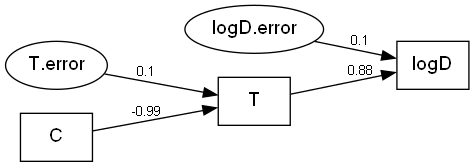
\includegraphics[width=4in]{Chap_7/path.png}
    \label{fig:Chap7_path_diagram}
\end{figure}

\begin{figure}[!ht]
    \caption[Simulated performance of a SEM when fitting a causal map]{Estimates of the covariate effects and predictive performance; see Fig. \ref{fig:Chap7_GLM_performance} caption for details and note the smaller x-axis range for tree cover and temperature-effect estimates.}
    \centering
    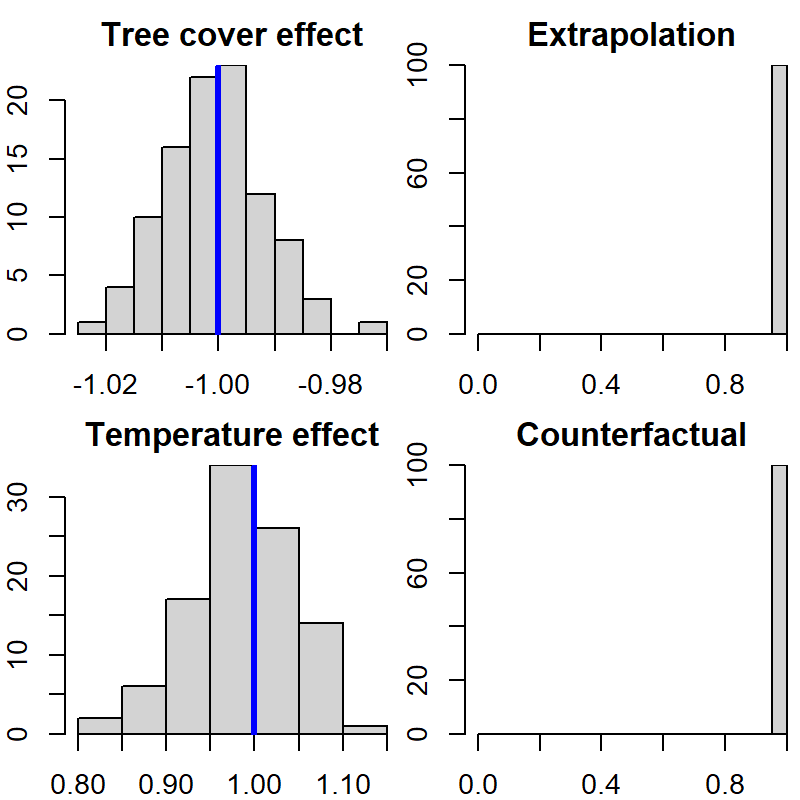
\includegraphics[width=4in]{Chap_7/SEM_performance.png}
    \label{fig:Chap7_SEM_performance}
\end{figure}

To fit this SEM using a log-linked Poisson distribution for soil invertebrate counts, we:
\begin{enumerate}
    \item specify a multivariate normal distribution for three variables; and 

    \item specify how those three variables are linked to measurements, e.g., where \(C\) and \(T\) are assumed to be measured without error (and hence are mapped to their observed values), while \(N\) is specified to follow the a Poisson distribution with log-intensity \(\log(D)\). 
\end{enumerate}
Fitting this model to the same data set as Fig. \ref{fig:Chap7_causal_map}, we see that a generalized SEM results in an accurate estimate of the link between tree cover and temperature, as well as between temperature and densities (Fig. \ref{fig:Chap7_path_diagram}).  Replicating this experiment one-hundred times, we also see that the model has highly precise estimates of each effect, and also has similar performance for both extrapolation and counter-factual prediction (Fig. \ref{fig:Chap7_SEM_performance}).  This similar performance shows that the SEM has addressed the changing structure of collinearity during counter-factual prediction by correctly specifying the relationship among variables \cite{dormann_collinearity_2013}.

We therefore conclude that properly specifying the mechanistic associations among covariates permits accurate predictions both when covariates follow the same process as sampling data, and when exogenous drivers cause covariates to differ systematically from their relationship in available sampling data.  Usefully, this SEM reduces to a familiar GLM when the user defines one variable as a response and the others as predictors, i.e., by specifying that all mechanisms involve an effect of each predictor on the response.  This confirms that a GLM will perform well for counterfactual prediction if there is no mechanistic association among covariates.  

However, we note that SEM does not resolve all problems regarding causal inference.  We instead use SEM as a simple example of the larger universe of models that can be constructed and interpreted using do-calculus. In particular, SEM has the following limitations:
\begin{itemize}
    \item \textit{Linearity}:  SEM assumes that causal mechanisms are well approximated by a linear response.  However, ecological systems often have thresholds and saturating relationships, and these are presumably not well described by SEM.  These circumstances then require developing a nonlinear approach, e.g., using a path diagram that involves generalized additive models;

    \item \textit{Dependence on specified causal map}:  more generally, both SEM and do-calculus generally will only yield unbiased estimates if the causal map represents real-world mechanisms.  If additional mechanisms occur in nature but are not modeled, then the estimates of direct and indirect effects will likely be both biased and inconsistent.
\end{itemize}
In summary, we recommend more development of causal methods in statistical ecology.  We also acknowledge that fundamental challenges remain when analyzing observational data to infer mechanistic relationships among variables.  In particular, the dependence on the specified causal map implies that ecologists must continue to use experimental field and laboratory methods to inform the structure among covariates that is assumed when analyzing observational data \cite{ives_random_2022, thorson_grand_2021}.  

\section{Benefits of Density Covariates}

We next demonstrate the potential benefit of including covariates when estimating total abundance from spatially representative sampling designs (a.k.a., interpolation).  As we saw in Section \ref{sec:Chap7_predicting_effect}, this predictive task is less dependent upon correctly specifying the association among covariates than counter-factual prediction.  We therefore proceed with the conventional regression-model assumption that covariates are exogenous and independent.  We also explore the case of a well-known model, e.g., the log-Gaussian Cox process from Section \ref{sec:Chap2_GLMM}.

We specifically use the mainland territory of Finland as the spatial domain, and overlay a square grid with dimensions 0.5 latitude by 0.5 longitude, which results in 271 grid-cells.  We use this domain to define a Conditional Autogressive (CAR) model assuming rook-adjacency (see Section \ref{sec:Chap5_CAR}), and simulate two latent variables \(\mathbf{x}_1\) and  \(\mathbf{x}_2\) that each follow a multivariate normal distribution:  

\begin{equation}
\begin{gathered}
  \mathbf{x}_1 \sim \mathrm{MVN}(\mathbf{0}, \sigma_1^2 \mathbf{Q}^{-1} ) \\
  \mathbf{x}_2 \sim \mathrm{MVN}(\mathbf{0}, \sigma_2^2 \mathbf{Q}^{-1} ) \\
  \log(\lambda_s) = \beta_0 + x_{i,1} + x_{i,2} \\
  c_s \sim \mathrm{Poisson}( \lambda_s )
\end{gathered}
\end{equation}
where \( \mathbf{Q} = \mathbf{I} - \rho \mathbf{A} \) and \(\mathbf{A}\) is the rook adjacency matrix and we simulate \(\rho\) at 75\% of the maximum admissible value (i.e., 0.75 times the maximum eigenvalue for \(\mathbf{A}\)).

We then estimated parameters by fitting a similar model structure as was used to simulate data:

\begin{equation}
\begin{gathered}
  \mathbf{\omega} \sim \mathrm{MVN}(\mathbf{0}, \sigma_{\omega}^2 \mathbf{Q}^{-1} ) \\
  \log(\lambda_s) = \beta_0 + \omega_{i} + \mathbf{x}_{i} \mathbf{\gamma} \\
  c_s \sim \mathrm{Poisson}( \lambda_s )
\end{gathered}
\end{equation}
where \(\mathbf{\omega}\) is treated as a random effect, and we can supply some combination of \(\mathbf{x}_1\) and \(\mathbf{x}_2\) as covariate matrix \(\mathbf{X}\) while estimating the appropriate number of response coefficients \(\mathbf{\gamma}\).

To illustrate simple properties of this model, we first test performance under the scenario that one sample is available from each grid-cell, that we have no covariates available (i.e., \(\mathbf{X}\) is a matrix with zero columns), and explore performance for estimating the area-weighted total density, \(\sum_s^{n_s} \lambda_s \).  We have two hypotheses about model performance:
\begin{itemize}
    \item \textit{Unbiasedness}:  given that the same model is used for simulation data and estimating parameters, we hypothesize that the epsilon bias-correction estimator will result in an unbiased estimate of area-weighted total abundance;

    \item \textit{Poisson-distribution for standard error}:  if we were fitting a model in which \(\omega_s\) was estimated independently for each site \(s\), then the predictive variance for each site would be \(c_i\).  Similarly, because the sum of Poisson distributions is itself Poisson-distributed, and defining the sum \(  c_{total} = \sum_s^{n_s} c_s \), then the area-weighted total abundance should have predictive variance of approximately \( c_{total} \).  We therefore hypothesize that the standard error for predictive total abundance will be approximately \(\sqrt{c_{total}}\) when the model does not account for spatial autocorrelation.
\end{itemize}
A single replicate of the simulation is consistent with both assumptions, e.g., where the epsilon bias-corrected estimate is within one standard error of the true value, and the standard error is very close to the square-root of true total abundance.

%\verbatiminput{Chap_7/check_hypotheses.txt}
\lstset{style=Routput}
\lstinputlisting[language=R]{Chap_7/check_hypotheses.txt}

We next move on to more complicated properties of this model.  Specifically, if we only have samples available for a small subset of grid-cells, then estimating the total abundance will involve interpolation and standard errors will be substantially larger than in the case where samples are available for all grid cells.  However, how will including one or both covariates affect the standard error of this estimate?

\begin{figure}[!ht]
    \caption[Simulation experiment comparing SDM with and without covariate]{Relative error in epsilon bias-corrected estimate of total abundance (left panel) and estimated standard error (right panel) when either including \(\mathbf{x}_1\) as a covariate or not (blue and red, respectively), showing a boxplot that summarizes 100 simulation replicates for each.}
    \centering
    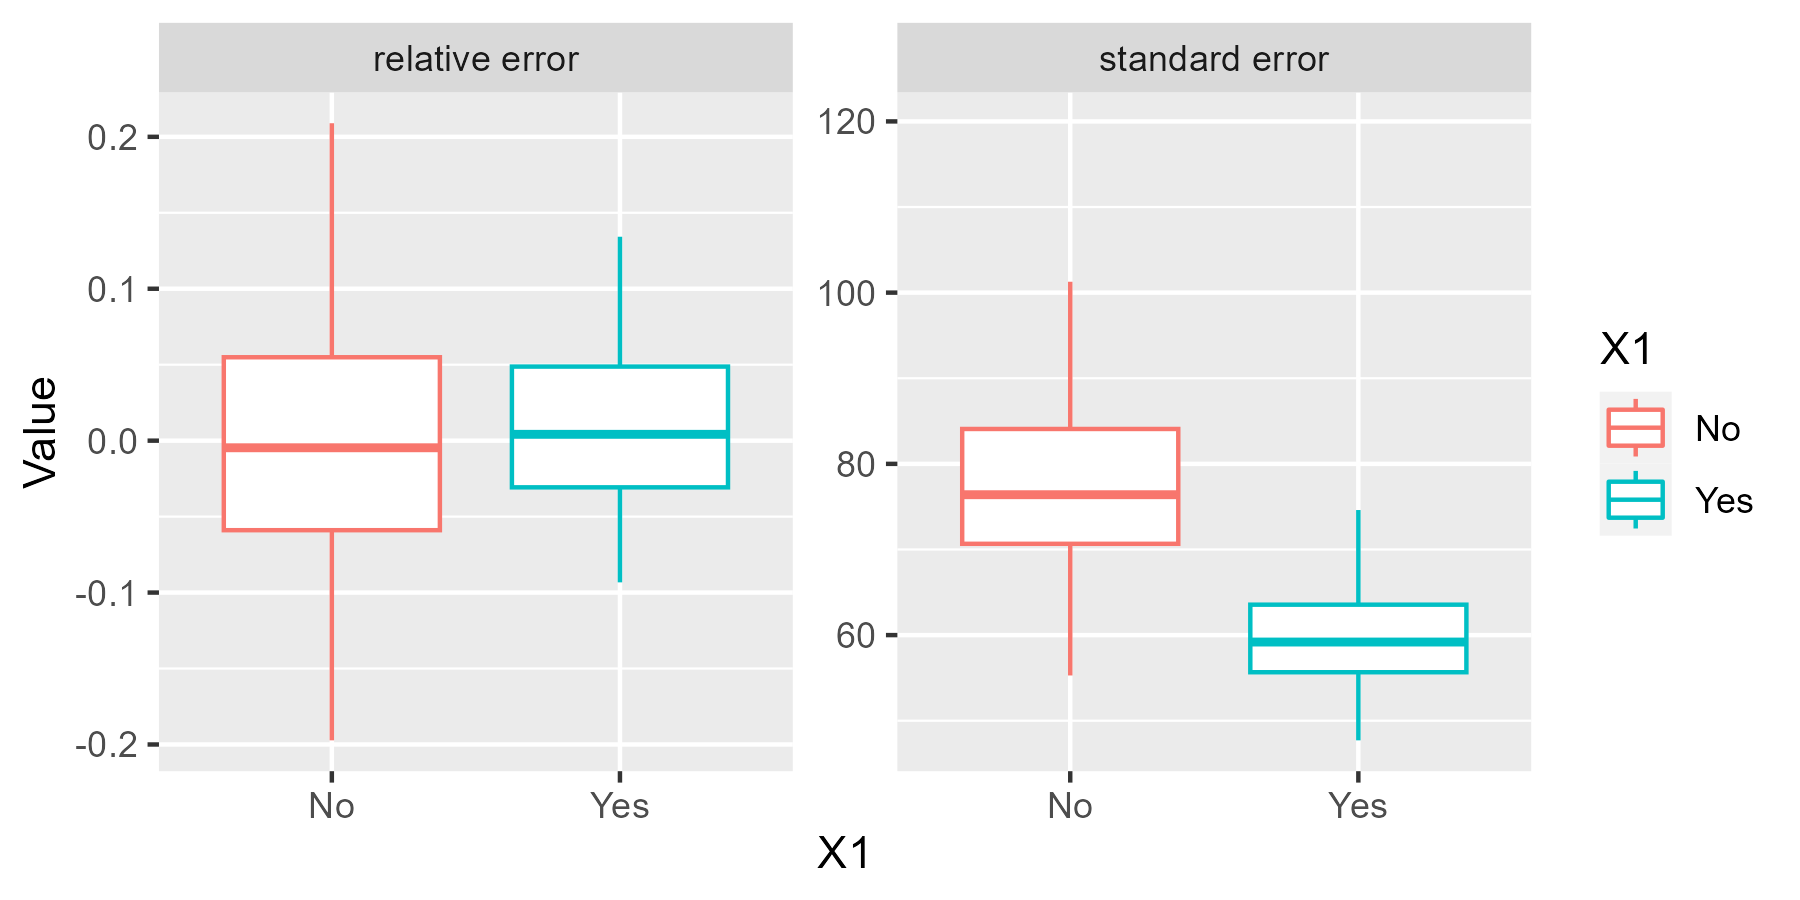
\includegraphics[width=5.5in]{Chap_7/Simulation_results.png}
    \label{fig:Chap7_simulation_results}
\end{figure}

To explore this, we simulate 100 replicates of an experiment.  For each replicate, we simulate the same model, but with \(\mathbf{x}_1\) explaining a larger portion of the variance than \(\mathbf{x}_2\), i.e., \(\sigma_1^2=0.6^2\) and \(\sigma_2^2=0.3^2\), and we also only simulate 100 grid-cells being sampled. For each replicate, we then fit two models model, either (1) not using covariates at all, or (2) using \(\mathbf{x}_1\) as a covariate.  For each replicate, we then extract the relative error in estimated total abundance, and the estimated standard error for estimated total abundance.  Results confirm that the epsilon bias-corrected estimate of total abundance is approximately unbiased either with or without including \(\mathbf{x}_1\) as covariate.  However, including \(\mathbf{x}_1\) as a covariate decreases the interquartile range for relative error and also decreases the average standard error for total abundance by approximately 20\% (Fig. \ref{fig:Chap7_simulation_results}).

From these two exercises involving a log-Gaussian Cox process, we therefore conclude that we can obtain an approximately unbiased estimate of total abundance with either complete or partial sampling of a spatial domain, and that including an informative covariate can decrease the standard error in an estimate of total abundance.  

\section{Density and Detectability Covariates} \label{sec:Chap7_covariates}

Finally, we introduce a basic distinction between density and detectability covariates:

\begin{enumerate}
    \item \index{density covariates}\textit{Density covariates} are measurements that can be fitted as a predictor variable in a regression, where a change in the covariate is associated with a corresponding change in the target variable (e.g., population density in a species distribution model).  As a consequence, predicting the expected value for the target variable at location \(s\) should be done conditional upon the values of density covariates at that location;

    \item \index{detectability covariates}\textit{Detectability covariates} are also measurements that can be fitted as predictor variable, but where changes in the covariate are not associated with changes in the target variable.  Instead, these detectability covariates are associated with changes in the expected measurement, but believed to not indicate changes in the target variable itself.  These detectability covariates typically include categorical variables indicating different sampling methods and other characteristics of sampling.     
\end{enumerate}
This distinction may seem obvious.  However, different research communities often implicitly assume that all covariates are either habitat or detectability, and results will differ greatly depending upon this assumption.  For example, \textit{index standardization} in fisheries science has historically included covariates to control for differences in sampling and has conventionally involved interpreting estimates of an annual intercept as representing changes in population density \cite{beverton_dynamics_1957}.  Therefore, fitting covariates explains variance that might otherwise be attributed to the annual intercept.  This treatment implicitly assumes that all covariates affect detectability, including variables like ocean temperature that in reality likely drive changes in population density itself.  By contrast, species distribution models typically use the same set of variables when fitting the model and when predicting density at new locations.  This treatment involves the implicit assumption that covariates affect population density rather than detectability, despite the fact that density covariates (e.g., tree cover) might affect sampling efficiency.

The simplest form of detectability covariate is an \myindex{offset variable}.  For example, an analyst might model population density using a log-linked generalized linear model but where each measurement \(C_i\) resulted from sampling density over a spatial area \(\mathcal{A}_i\) with area \( a_i = |\mathcal{A}_i|\).  In this case, expected density \( \E(C_i) \propto a_i \lambda_i \), or using GLM notation:

\begin{equation}
    \log \left(\E(C_i) \right) = \beta_0 + \omega_i + \log(a_i)
\end{equation}
where \(e^{\beta_0}\) is the proportionality constant (i.e., detectability from Section \ref{sec:Chap6_occupancy_model}), \(\omega\) is other spatial terms, and \(\log(a)\) represents the assumed linear scaling of the sample expectation with sample area.  

To further demonstrate this distinction between density and detectability covariates, we also introduce the concept of an \myindex{integrated model}.  We define an integrated model as one that is fitted to multiple data types and/or sources, which all measure an ecological variable but also differ in other respects.  In this case, we estimate biomass density \(D = N W\) (with units kilograms per area), defined as the product of numerical density \(D\) (with units numbers per area) and average weight \(W\) (with units kilograms per number).  Samples of biomass \(B\) directly measure \(D\), while counts \(C\) directly measure \(N\).  We also introduce the the \myindex{complementary log-log link function} (see Section \ref{sec:Appendix_links_and_distributions}).  Under the assumption that \(C\) individuals are present in the vicinity of sampling and that this count follows a Poisson distribution \(C \sim \mathrm{Poisson}(N)\), the probability of having at least one individual present, \( \Pr(C>0) = \pi = 1 - e^{-N} \).  Assuming that we directly model log-abundance, this then results in a cloglog link function, which can transform encounter probability \(\pi\) to a linear predictor \(p\):

\begin{equation} \label{eq:Chap7_cloglog}
  \mathrm{cloglog}(\pi) = \mathrm{log}( - \mathrm{log}(1 - \pi)) = p
\end{equation}
where \(p = \mathrm{log}(N)\) is the modeled linear predictor for log-abundance, or equivalently the inverse-cloglog function:

\begin{equation} \label{eq:Chap7_clogloginv}
  \mathrm{cloglog}^{-1}(p) = 1 - e^{-e^p} = \pi
\end{equation}
where this inverse-link transforms a linear predictor \(p\) to the expected encounter probability \(\pi\).
 
Given this brief derivation of the cloglog link function, we next define a specific distribution for each of three types of data (see Section \ref{sec:Appendix_links_and_distributions})
\begin{itemize}
    \item \textit{Biomass}:  we specify that biomass-sampling data follows a Tweedie distribution:

\begin{equation}
    B \sim \mathrm{Tweedie}( D, \phi, \psi )
\end{equation}

   where \(\phi\) and \(\psi\) are parameters that represent the variance of samples, \(\mathrm{var}(Y)= \phi D^{\psi} \). This Tweedie describes a compound Poisson-gamma process whenever \(1 < \psi < 2\) (recalling Section \ref{sec:Chap2_compound_distribution}), i.e., where we sample a count from a Poisson distribution, and then each individual has weight that follows a gamma distribution;  

   \item \textit{Counts}:  similarly, we specify that count data follow a Poisson distribution:
   
\begin{equation}
    C \sim \mathrm{Poisson}( \eta_1 D )  
\end{equation}

   where \( \eta_1 \) is the log-ratio of expected counts and expected biomass samples at the same place and time, which captures different sampling efficiency as well as the conversion \(W\) from weight to numbers;

   \item \textit{Encounters}:  finally, we specify that binary encounter/non-encounter data follow a Bernoulli distribution using a complementary log-log link function:

\begin{equation}
    E \sim \mathrm{Bernoulli}\left( 1 - e^{-\eta_2 D} \right) 
\end{equation}

   where \(E\) is a binary 0/1 indicator indicating whether or not the species was encountered in a sample, and \( \eta_2 \) similarly converts from biomass to encounter-rate data.  
\end{itemize}
This model has been explored previously \cite{gruss_developing_2019}, and we follow that paper in fitting it to samples of red snapper (\textit{Lutjanus campechanus}) in the United States waters of the Gulf of Mexico.  We specifically fit biomass samples from the a bottom trawl survey (the SEAMAP Groundfish Trawl Survey), count data from an accoustic and midwater trawl survey (the National Marine Fisheries Service Pelagic Acoustic Trawl Survey), and encounter/non-encounter data from a longline survey (the NMFS Red Snapper/Shark Bottom Longline Survey)\footnote{Data are publicly available as file ``multimodal\_red\_snapper\_example.rda" downloaded with R-package VAST \cite{thorson_guidance_2019}, and thank Arnaud Gruss for compiling these data in support of a previous publication \cite{gruss_developing_2019}.}.  We also obtain data regarding the depth of the seafloor below the ocean surface (termed \textit{bathymetric depth}), using the ETOPO 2022 data \cite{noaa_national_centers_for_environmental_information_etopo_2022} downloaded using R-package \colorbox{backcolour}{marmap} \cite{pante_marmap_2020}.  We treat calendar year and bathmetric depth as density covariates, and specify a quadratic basis expansion to bathymetric depth so that we can estimate any optimum in the estimated bathymetric response function (see Section \ref{sec:Chap5:splines}).     

Expressing this integrated model in full, we arrive at the following specification:

\begin{equation}
\begin{gathered}
  p_i = \omega_{s_i} + \mathbf{x}_i \mathbf{\gamma} + \mathbf{q}_i \mathbf{\eta} \\
  \mathbf{\omega} \sim \mathrm{MVN}( \mathbf{0}, \sigma^2 \mathbf{Q}^{-1} ) \\
  y_i \sim
 \begin{cases}
    \mathrm{Tweedie}( \mathrm{log}^{-1}(p_i), \phi, \psi ) & \text{if } y_i \text{ samples biomass} \\
    \mathrm{Poisson}( \mathrm{log}^{-1}(p_i) ) & \text{if } y_i \text{ samples counts} \\
    \mathrm{Bernoulli}( \mathrm{cloglog}^{-1}(p_i) )  & \text{if } y_i \text{ samples encounter/non-encounter}
  \end{cases}
\end{gathered}
\end{equation}
where \(\mathbf{x}_i\) is the vector of density covariates co-located with sample \(i\), and \(\mathbf{q}_i\) is the vector of detectability variables for sample \(i\).  In practice, this model can be implemented in TMB while using input vector \colorbox{backblue}{e\_i} to indicate whether a given sample arises from a biomass, count, or encounter/non-encounter sample (Code \ref{code:Chap7-integrated-model}). We use the SPDE method to assemble a sparse precision matrix from sparse matrices \colorbox{backblue}{M0}, \colorbox{backblue}{M1}, and \colorbox{backblue}{M2}, and again using the \colorbox{backblue}{density::GMRF} function to compute the negative log-likelihood from that distribution (as introduced in Section \ref{sec:Chap5_SPDE}).  

The main novelty in this code is the use of the TMB function \colorbox{backblue}{logspace\_sub} when applying the inverse-cloglog link function to compute the log-likelihood for Bernoulli-distributed samples.  This inverse-link function \(1-e^{-e^p}\) involves exponentiating the linear predictor and then exponentiating its negative value, and any sequence of exponential functions easily results in numerical under or overflow.  However, we want to calculate the log-density of the Bernoulli distribution resulting from computing the log of this inverse-link function.  We therefore use TMB code that evaluates \(\log(e^X-e^Y)\) without actually computing either \(e^X\) or \(e^Y\).  To do so, we define \(X=0\) and \(Y=-e^p\), and pass each to function \colorbox{backblue}{logspace\_sub}.  By doing so, we calculate the log of the inverse cloglog function while replacing two calls to an exponential function with only one. 

\lstset{style=TMBcode}
\lstinputlisting[language=c++, label=code:Chap7-integrated-model, caption=TMB code for an integrated species distribution model that is fitted to biomass counts and encounter/non-encounter data., captionpos=t]{Chap_7/integrated_model.cpp}
\label{code:Chap7_integrated_model}

To model detectability in this case study, we obtain an indicator variable (a.k.a. factor) that lists the sampling method for each sample, and convert this to an indicator matrix.  We then drop one column of this matrix to avoid specifying two intercepts (the first in density covariates \(\mathbf{X}\) and the second in catchability covariates \(\mathbf{Q}\)), which would then be confounded.  For example, this might result in a detectability matrix for three hypothetical samples (rows):

\begin{figure}[!ht]
    \caption[Predicted density of red snapper from an integrated model]{The spatial distribution of biomass, count, and encounter/non-encounter samples (top panel) fitted by an integrated model for red snapper in the Gulf of Mexico overlaid on the modeled spatial domain (grey polygon), as well as predicted log-biomass density (middle panel), and the standard error in log-biomass density (bottom panel) obtained from sampling the joint precision of fixed and random effects (Section \ref{sec:Chap6_sample_joint_precision}), where the latter two only show log-density or standard errors for locations with density greater than 0.1\% of the maximum value (and other areas are displayed as grey) to allow greater visual contrast for areas that are plotted.}
    \centering
    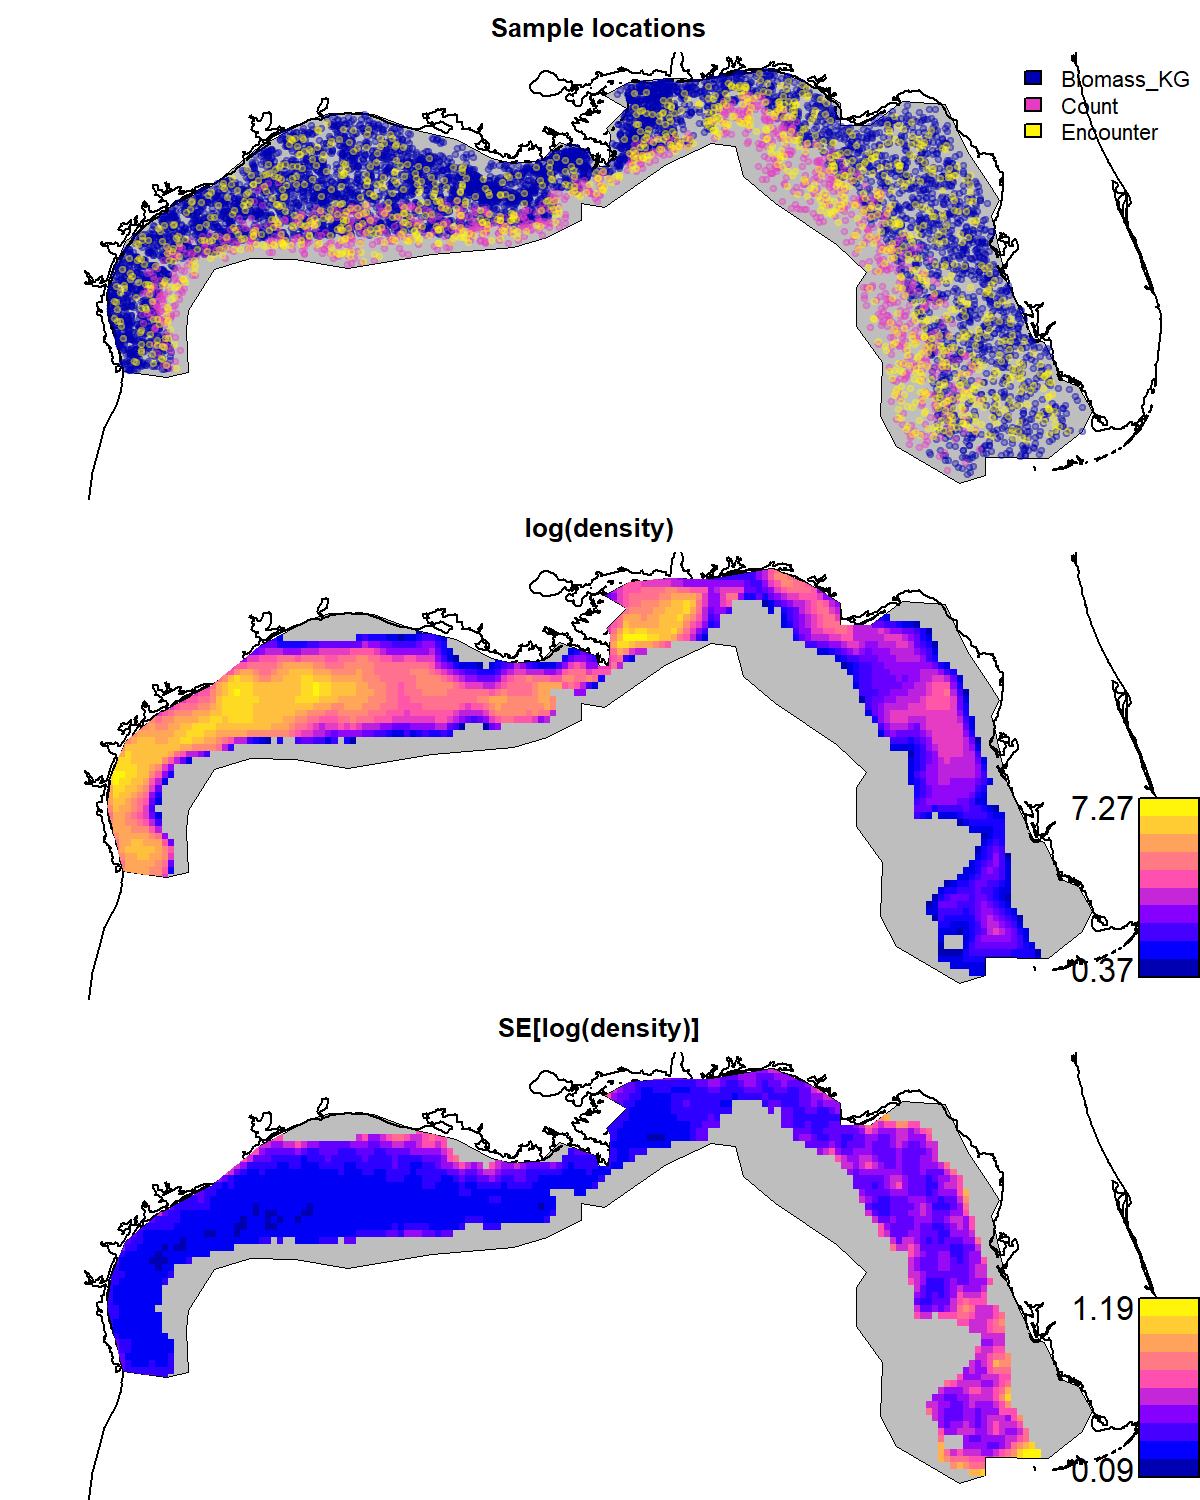
\includegraphics[width=5.5in]{Chap_7/Predicted densities.png}
    \label{fig:Chap7_predicted_densities}
\end{figure}

\begin{equation} \label{eq:Chap7_Q}
    \mathbf{Q} = \begin{bmatrix}
    0 & 0 \\
    1 & 0 \\
    0 & 1 \\
    \end{bmatrix} 
\end{equation}
where the first row corresponds to a biomass sample, the second row to a count, and the third row to a sample of encounter/non-encounter data, such that \(\eta_1\) is the detectability coefficient for counts relative to biomass samples, and \(\eta_2\) is the detectability coefficient for encounter/non-encounter data relative to biomass samples.  

\begin{figure}[!ht]
    \caption[Estimated covariate responses from an integrated model]{The estimated effect of bathymetry on biomass density for red snapper (left panel) when fitting a quadratic response as a density covariate, and the estimate of the annually varying intercept for each year with available data (right panel), where each shows a 95\% confidence interval.}
    \centering
    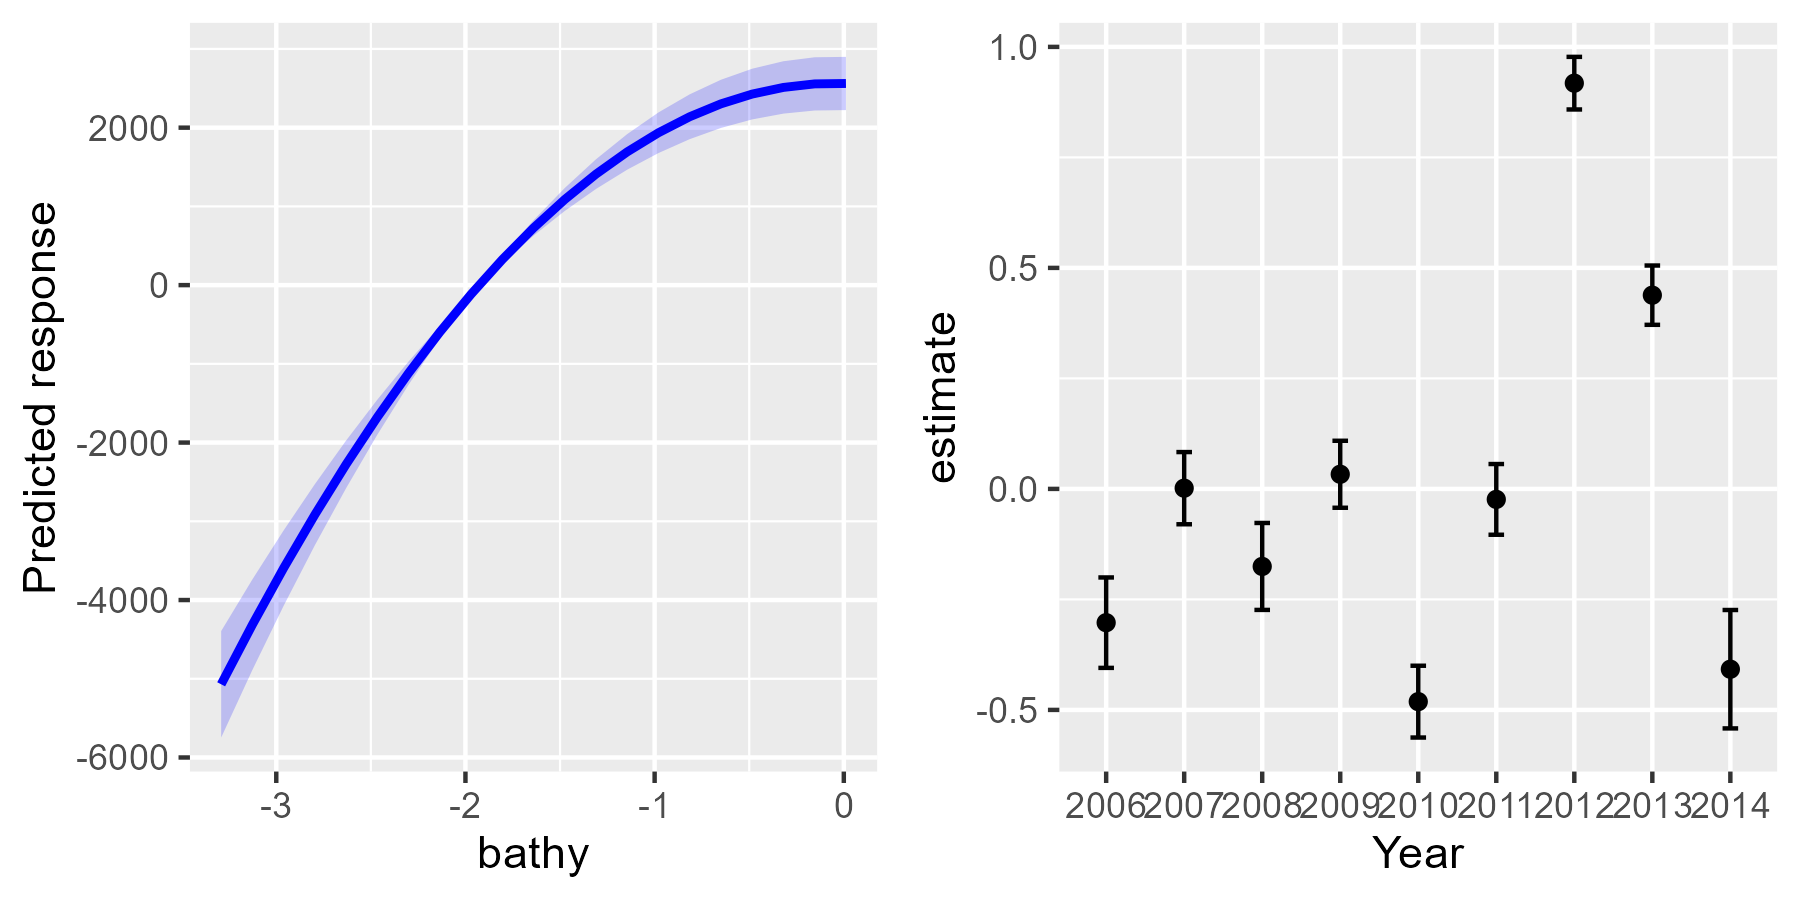
\includegraphics[width=5.5in]{Chap_7/covariate_response.png}
    \label{fig:Chap7_covariate_response}
\end{figure}

Fitting this integrated model to these three types of data, we estimate that red snapper has highest densities in inshore areas from Texas through immediately east of the Mississippi delta, with lower densities offshore and particularly in the Western Florida shelf (Fig. \ref{fig:Chap7_predicted_densities}).  Predictions have a coefficient of variation of approximately 6--10\% throughout much of this area, with higher uncertainty in areas with lower density.  This relationship (where standard error decreases where densities are higher) presumably results from the specified distributions for sampling, where the standard deviation of sampling decreases with increased mean for the Poisson and Tweedie distributions.  Similarly, we estimate that densities decline rapidly with increasing bathymetry, and identify higher median density in some years (e.g., 2012) than others (e.g., 2010), although there is little evidence of an overall trend in the estimated intercept values (Fig. \ref{fig:Chap7_covariate_response}).    

\section{Chapter Summary}

In summary, we have showed that:
\begin{enumerate}
    \item Covariates are included in spatio-temporal models for many different purposes, including (1) mitigating bias that would otherwise arise from ignoring differences in sampling methods or gears, (2) predicting densities in areas that resemble those that are sampled (termed interpolation), (3) attributing observed patterns to different covariates, and (4) predicting densities in conditions that are different than those that are sampled (termed counter-factual prediction, and generally measuring transferability);  

   \item Attribution requires some inference about causality, and causality can be formally expressed using do-calculus, which involves predicting a change in one or more variables based explicitly on either endogenous mechanisms (i.e., the effect of a change in some other modeled variable) or exogenous mechanisms (i.e., an experimental treatment or novel condition).  Do-calculus involves defining a causal map, and if all mechanisms are linear then parameters can be estimated by fitting a structural equation model.  Replacing an explicit path diagram with a standard regression model (where all predictor variables have an immediate effect on a specified response variable) can still result in good predictive performance when interpolating density, but often will degrade performance when extrapolating density;

   \item Covariates can be broadly classified as either representing habitat (i.e., variables that are associated with local population density) or detectability (i.e., variables that measure a difference in sampling performance independently of local density).  Using point-count data, it is often necessary to determine whether a given variable affects density or detectability based on ecological and system knowledge.  When including both density and detectability variables, it is necessary to exclude an intercept from one or the other to avoid confounding;  

   \item Including density covariates can explain variance that would otherwise be attributed to a spatially correlated residual term.  By doing so, density covariates can substantially decrease the standard error for predictions of local density or spatially integrated abundance;  

   \item Integrated models typically involve fitting more than one type of data, where these data types are all informative about some variables and/or parameters but differ systematically in other respects.  For example, it is possible to fit biomass, counts, and encounter/non-encounter data jointly, particularly when using a complementary log-log link function to derive the encounter probability from numerical density.  
\end{enumerate}

\section{Exercises}

\begin{enumerate}
    \item In Eq. \ref{eq:Chap7_cloglog}, we introduce the complementary log-log link function and claim that the inverse cloglog can take as input the log-linked linear predictor \(p\) for a Poisson distribution \( C \sim \mathrm{Poisson}(e^p)\) and return the probability of an encounter, \(\Pr(C > 0)\).  Confirm that this claim is true, either analytically from the probability mass function for the Poisson distribution or numerically by simulating replicates from a Poisson distribution and calculating the resulting encounter frequency for different values of \(p\).   

    \item In Eq. \ref{eq:Chap7_sem_example}, we illustrated the challenges with extrapolation or counterfactual prediction when fitting a generalized linear model (GLM) to covariates that are not independent.  We further showed that a structural equation model (SEM) can incorporate information regarding the relationship among covariates to address these challenges.  However, we did not compare GLM and SEM performance in the case when GLMs are expected to perform well.  Change the data-generating process to incorporate independent covariates:

\begin{equation} \label{eq:Chap7_sem_exercise}
\begin{gathered}
   X \sim \mathrm{Normal}(0,1) \\ 
   Y \sim \mathrm{Normal}(0,0.5)  \\
   Z \sim \mathrm{Poisson}\left(e^{X+Y}\right)
\end{gathered}
\end{equation}

    We will continue to specify the SEM using the original specification (Eq. \ref{eq:Chap7_sem_example}), which no longer matches the true data-generating process.  Now repeat the simulation experiment using this alternative data-generating process, and compute extrapolation and counterfactual performance for both the GLM and SEM.  Does the GLM continue to have different performance for extrapolation and counterfactual prediction?  How does the SEM perform given that the structural assumptions are now mis-specified?

\end{enumerate}

